\documentclass[a4paper, 12pt]{article}

\def\languages{french, english}

%%%%%%%%%%%%%%%%%%% Libraries

\input{include/libraries/bibliography.tex}
\input{include/libraries/default.tex}
\input{include/libraries/figures.tex}
\input{include/libraries/informatics.tex}
\input{include/libraries/mathematics.tex}
\input{include/libraries/theorems.tex}
\input{include/libraries/units.tex}

\input{include/languages/french.tex}

%%%%%%%%%%%%%%%%%%% Additional packages

\usepackage{subcaption}

%%%%%%%%%%%%%%%%%%% Titlepage

\def\logopath{resources/pdf/logo-uliege.pdf}
\def\toptitle{University of Liège}
\title{Open Loop System}
\def\subtitle{Linear control systems}
%\def\authorhead{Author}
\author{
    Bastien \textsc{Hoffmann} (20161283)\\
    Maxime \textsc{Meurisse} (20161278)\\
    Valentin \textsc{Vermeylen} (20162864)\\
}
%\def\rightauthorhead{}
%\def\rightauthor{}
\def\context{Master in Civil Engineering}
\date{Academic year 2019-2020}

%%%%%%%%%%%%%%%%%%% Options

\fancyhead[R]{}
\renewcommand{\thesubsection}{\arabic{subsection}}
\addbibresource{references.bib}
\defbibheading{bibliography}[\refname]{}

%%%%%%%%%%%%%%%%%%% Document

\begin{document}
    % ----- Titlepage ----- %
    \input{include/titlepages/default.tex}
    
    % ----- Detailed schematic of the open loop system ----- %
    \subsection{Detailed schematic of the open loop system}
    The detailed schematic of the open loop studied system is shown in figure \ref{fig:detailed_schematic}.
    \begin{figure}[H]
        \centering
        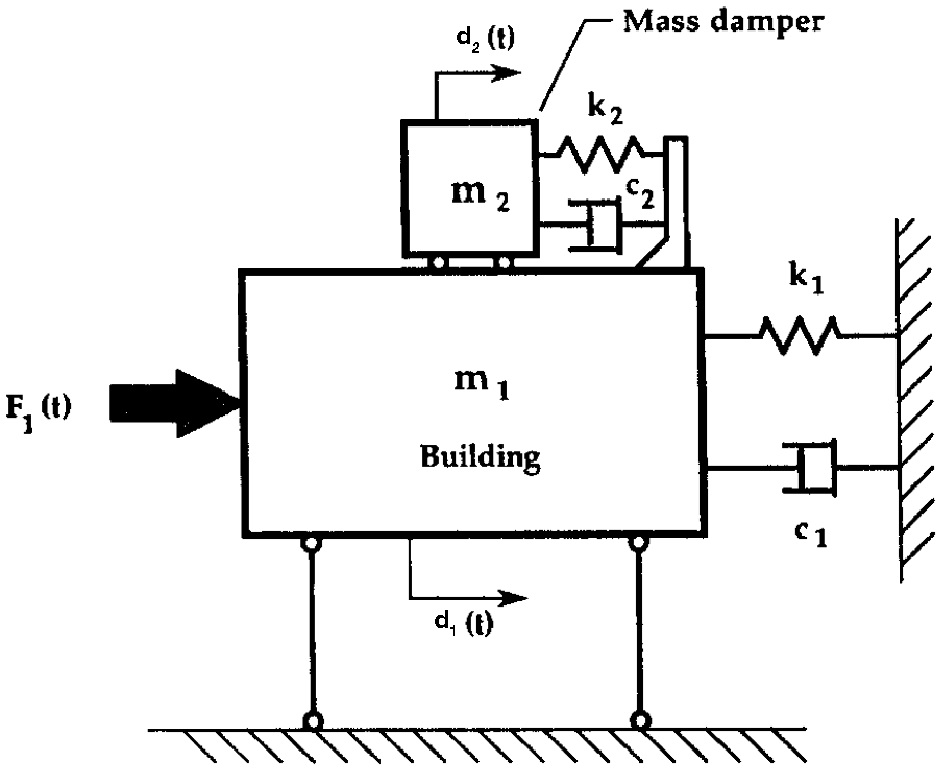
\includegraphics[width=0.7\textwidth]{resources/pdf/schema-without-controller.pdf}
        \caption{Detailed schematic of the open loop studied system \cite{science_direct}}
        \label{fig:detailed_schematic}
    \end{figure}
    The building is represented by the mass $m_1$ and its oscillation motion is simulated by the spring $k_1$ and the damper $c_1$.\par
    The mass damper is represented by the mass $m_2$ and its movement is simulated by the spring $k_2$ and the damper $c_2$.\par
    The force $F_1(t)$ represents the wind force (uncontrollable) on the building.
    
    % ----- Constraints, assumptions, limitations ----- %
    \subsection{Constraints, assumptions, limitations}
    To model and study the system, we defined a series of constraints, assumptions and limitations, presented in table \ref{tab:constraints_assumptions_limitations}.\par
    \begin{table}[H]
        \centering
        \begin{tabular}{|l|c|}
            \hline
            \multirow{2}{*}{{\bf Building}} & height of \SI{250}{\meter}, width of \SI{40}{\meter}\\ & movement along a single axis (horizontal)\\\hline
            {\bf Wind force} & max intensity of \SI{7.35}{\mega\newton}\\ \hline
            {\bf Mass} & no friction between $m_1$ and $m_2$\\ \hline
        \end{tabular}
        \caption{Constraints, assumptions and limitations of the system.}
        \label{tab:constraints_assumptions_limitations}
    \end{table}
    
    % ----- State-space representation ----- %
    \subsection{State-space representation}
    Input vector $U$ and state vector $X$ are given by :
    $$
    U = \begin{pmatrix}
        F_1 \\
    \end{pmatrix}
    \hspace{3cm}
    X = \begin{pmatrix}
        d_1 \\
        \dot d_1 \\
        d_2 \\ 
        \dot d_2 \\
    \end{pmatrix}
    $$
    
    % Inputs
    \subsubsection{Inputs}
    $F_1(t)$, the force of the wind (uncontrollable).
    
    % Outputs
    \subsubsection{Outputs}
    $y = d_1(t)$ the relative position of the building with respect to the vertical position.
    
    % States
    \subsubsection{States}
    \begin{itemize}
        \item $x_1 = d_1$, as described above.
        \item $x_2 = \dot d_1$, the speed of the building.
        \item $x_3 = d_2$, the absolute displacement of the mass damper.
        \item $x_4 = \dot d_2$, the speed of the mass damper.
    \end{itemize}
    
    % Output law
    \subsubsection{Output law}
    The output is one of the states : $y = x_1$.
    
    % Input law
    \subsubsection{Input law}
    The input law is given by \cite{science_direct} :
    \begin{align*}
        m_{1}\ddot{d}_{1} + c_{1}\dot{d}_{1} + k_{1}d_{1} &= c_{2}\dot{z} + k_{2}z + F_{1}(t)\\
        m_{2}\ddot{z} + c_{2}\dot{z} + k_{2}z &= -m_{2}\ddot{d}_{1}
    \end{align*}
    with $z = d_2 - d_1$.\par
    The system is \textbf{linear}. We can easily derive the ABCD matrices.
    $$
    A = \begin{pmatrix}
        0 & 1 & 0 & 0 \\
        \frac{-k_1-k_2}{m_1} & \frac{-c_2-c_1}{m_1} & \frac{k_2}{m_1} & \frac{c_2}{m_1} \\
        0 & 0 & 0 & 1 \\ 
        \frac{k_2}{m_2} & \frac{c_2}{m_2} & \frac{-k_2}{m_2} & \frac{-c_2}{m_2}\\
    \end{pmatrix}
    \quad
    B = \begin{pmatrix}
        0\\
        \frac{1}{m_1}\\
        0\\
        0\\
    \end{pmatrix}
    \quad
    C = \begin{pmatrix}
        1 & 0 & 0 & 0\\
    \end{pmatrix}
    \quad
    D = \begin{pmatrix}
        0\\
    \end{pmatrix}
    $$
    
    % ----- System simulations without controller ----- %
    \subsection{System simulations without controller}
    To simulate the system, we choose a series of numerical values, presented in table \ref{tab:numerical_values} \cite{science_direct_2}.
    \begin{table}[H]
        \centering
        \begin{tabular}{|l|c|c|}
            \hline
            {\bf Mass} & $m_1$ = \SI{20000}{\tonne} & $m_2$ = \SI{10}{\tonne}\\ \hline
            {\bf Spring} & $k_1$ = \SI{1500}{\mega\newton/\meter} & $k_2$ = \SI{3.5}{\mega\newton/\meter}\\ \hline
            {\bf Damper} & $c_1$ = \SI{30}{\mega\newton\second/\meter} & $c_2$ = \SI{1}{\mega\newton\second/\meter}\\ \hline
        \end{tabular}
        \caption{Numerical values of the system}
        \label{tab:numerical_values}
    \end{table}
    For the strength of the wind, we considered 2 cases (in newton) :
    \begin{align*}
        F_1 &= \num{7350000} & \text{Constant wind force}\\
        F_1(t) &= \num{3675000}\sin(2\pi t) + \num{3675000} & \text{Sinusoidal wind force}
    \end{align*}
    These values have been approximated via
    \begin{equation*}
        F = \frac{1}{2}\rho v^2A
    \end{equation*}
    with
    \begin{itemize}
        \item $\rho$, the air density;
        \item $v$, the wind speed;
        \item $A$, the area of one side of the building.
    \end{itemize}
    \paragraph{Remark} We used SI units except for the newton we left as such.
    \begin{figure}[H]
        \centering
        \begin{subfigure}{0.495\textwidth}
            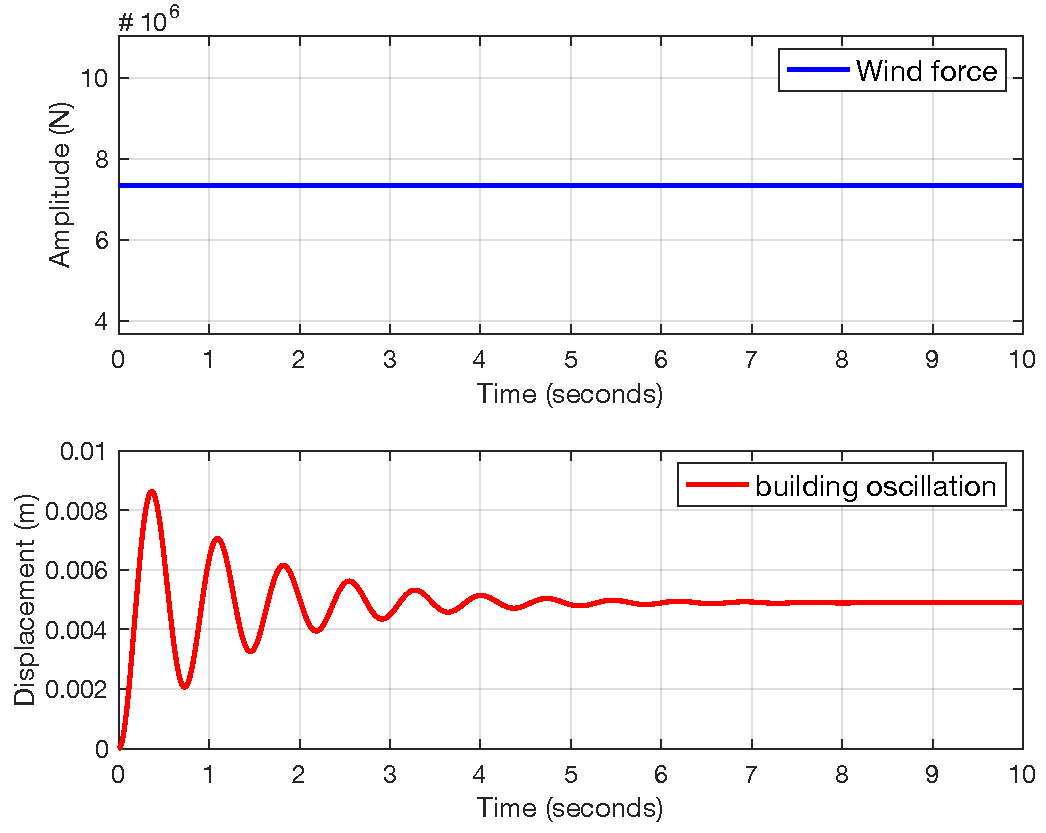
\includegraphics[width=\textwidth]{resources/pdf/constant.pdf}
            \caption{Constant wind force}
        \end{subfigure}
        \begin{subfigure}{0.495\textwidth}
            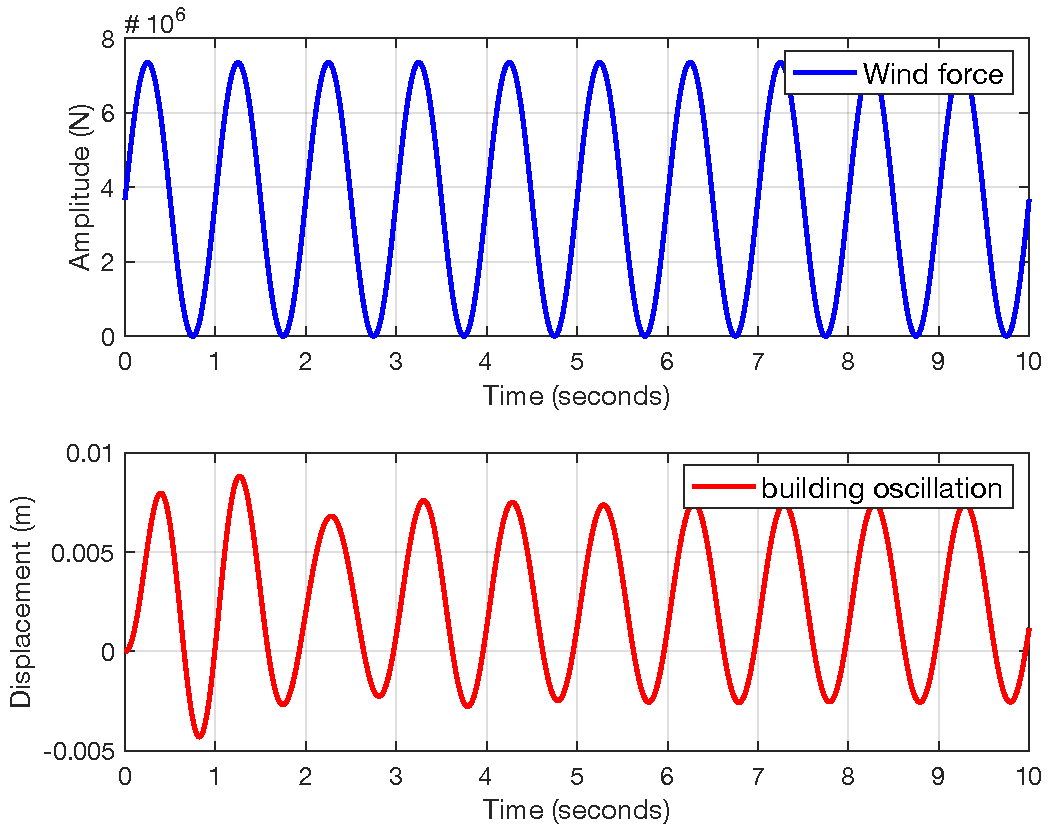
\includegraphics[width=\textwidth]{resources/pdf/sinusoidal.pdf}
            \caption{Sinusoidal wind force}
        \end{subfigure}
        \noskipcaption{Linear simulations results}
        \label{fig:simulations}
    \end{figure}
    In both cases, we observe that the building oscillates slightly at first and then moves according to the wind (in the first case, the building stabilises in an unbalanced position, and in the second case, the building oscillates steadily).
    
    % ----- State-space representation analysis ----- %
    \subsection{State-space representation analysis}
    
    % Stability
    \subsubsection{Stability}
    To study the stability of the system, we compute the eigenvalues of the dynamic matrix $A$ thanks to Matlab function (\texttt{eig}).\par
    The system is stable if the real parts of the eigenvalue are all negative. In the case of the studied system, we obtain the following eigenvalues :
    \begin{equation*}
        \lambda_i = \begin{bmatrix}
            \num{-96.4185}\\\num{-0.7498+8.6255i}\\\num{-0.7498-8.6255i}\\\num{-3.6319}
        \end{bmatrix}
    \end{equation*}
    Given these values, the system is stable.
    
    % Observability
    \subsubsection{Observability}
    To determine whether or not the system is observable, we compute the observability matrix thanks to Matlab function (\texttt{obsv}) :
    \begin{equation*}
        Ob = \begin{pmatrix}
            1 & 0 & 0 & 0\\
            0 & 1 & 0 & 0\\
            \num{-75.1750} & \num{-1.5500} & \num{0.1750} & \num{0.05}\\
            \num{134.0213} & \num{-67.7725} & \num{-17.7712} & \num{-4.9025}
        \end{pmatrix}
    \end{equation*}
    This matrix is full rank (verified with Matlab), the system is thus fully observable.
    
    % Controllability
    \subsubsection{Controllability}
    To determine whether or not the system is controllable, we compute the controllable matrix thanks to Matlab function (\texttt{ctrb}) :
    \begin{equation*}
        Co = \num{1e-8}\begin{pmatrix}
            0 & 5 & \num{-7.75} & \num{-338.862}\\
            5 & \num{-7.75} & \num{-338.862} & \num{-1255.906}\\
            0 & 0 & \num{500} & \num{-49024.99}\\
            0 & \num{500} & \num{-49024.99} & \num{4690900}
        \end{pmatrix}
    \end{equation*}
    This matrix is full rank (verified with Matlab), the system is thus fully controllable.
    
    % ----- Reference ----- %
    \newpage
    \subsection{Reference}
    \nocite{*}
    \printbibliography
\end{document}
